
\documentclass[12pt,a4paper]{article}

\usepackage[utf8]{inputenc}
\usepackage[T1]{fontenc}
\usepackage{lmodern}            % clean, well-proportioned fonts (pdflatex-safe)
\usepackage{microtype}         % better justification
\usepackage[a4paper,margin=1in]{geometry} 
\usepackage{parskip}           % space between paragraphs, no indent
\usepackage{graphicx}
\usepackage{float}
\usepackage{booktabs}

\usepackage{titlesec}
\usepackage{fancyhdr}
\usepackage{caption}
\captionsetup{font=small,labelfont=bf}
\usepackage[hidelinks]{hyperref}
\usepackage{xcolor}
\usepackage[normalem]{ulem}
% ----- STYLING -----
\renewcommand{\familydefault}{\rmdefault} % serif body for a formal look
\usepackage[utf8]{inputenc}
\usepackage[T1]{fontenc}
\usepackage{lmodern}
\usepackage{tcolorbox} % For title box
\usepackage{titling}   % For custom title formatting
\newtcolorbox{titlebox}{
  colback=blue!5,
  colframe=blue!40,
  boxrule=0.95pt,
  arc=6pt,
  auto outer arc,
  boxsep=6pt,
  left=10pt,
  right=10pt,
  top=10pt,
  bottom=10pt,
  colbacktitle=white,
  coltitle=black,
  center title
}


% Redefine maketitle
\pretitle{\begin{center}\begin{titlebox}\LARGE\bfseries}
\posttitle{\end{titlebox}\end{center}}
\preauthor{\begin{center}\large}
\postauthor{\end{center}}
\predate{\begin{center}}
\postdate{\end{center}}

\title{\textit{Biweekly Report 3 }\\[0.5em]
Improving the dynamic comparison framework and theorising digital organisms}
\author{Raunak Narwal\\
Department of Mathematical Sciences \\
Indian Institute of Science Education and Research, Mohali, 130406, Punjab}

\date{ October 24, 2025}

% Section spacing and look
\titleformat{\section}{\large\bfseries}{\thesection}{1em}{}
\titleformat{\subsection}{\normalsize\bfseries}{\thesubsection}{1em}{}
\titlespacing*{\section}{0pt}{1.2\baselineskip}{0.4\baselineskip}
\titlespacing*{\subsection}{0pt}{0.9\baselineskip}{0.25\baselineskip}

% Header / footer (minimal)
\pagestyle{fancy}
\fancyhf{}
\renewcommand{\headrulewidth}{0pt}
\fancyhead[L]{\small Biweekly Report III}
\fancyhead[R]{\small Raunak Narwal}
\fancyfoot[C]{\small Page \thepage}\setlength{\footskip}{20pt}


% Utility for graphics with special filenames
\newcommand{\imgfile}[1]{\detokenize{#1}}

% ----- DOCUMENT -----
\begin{document}
\maketitle
\vspace{-0.8em}
\hrule
\vspace{1.0em}

% Recommended line spacing: slightly tighter than 1.5 but more airy than single
\setlength{\parskip}{0.6\baselineskip}

\section*{General Modular Framework and how to run the files on local machine}
We integrated the two files, computing topological similarity and dynamic comparison, into a single automated workflow, \textit{runall.py}. This script takes two network files (in \textit{.kgml} or \textit{.csv}) as input and runs both persistence and dynamic analyses. For all the uses one can type python \textit{runall.py} to see the help.
\begin{figure}[H]
    \centering
    % replace with your image filename; \imgfile keeps special characters safe
    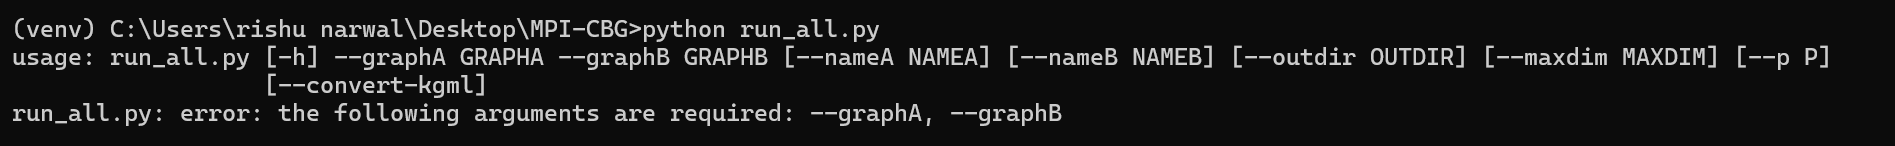
\includegraphics[width=1\linewidth]{Screenshot 2025-10-18 190034.png}}
    % caption intentionally left minimal
\end{figure}
To run the files on your local machine, clone this repository \href{https://github.com/RaunakNarwal735/Persistent-Homology}{here}, then run the following commands on your command prompt.
\begin{verbatim}
.venv\scripts\activate
pip install -r requirements.txt
python run_all.py --graphA --graphB --outdir
\end{verbatim}
\section*{Improving the Dynamic Comparison framework}
Our current dynamic comparison framework provides a simplistic functional baseline for simulating and comparing the behavior of two networks, it makes several simplifying assumptions that could limit its biological realism, current limitations include simplified reaction kinetics, all our reactions are currently happening with a rate constant of 1, assuming uniform first order kinetics, this oversimplifies the system. Incomplete Stoichiometry representation, each reaction decreases substrate concentration and increase the product concentration by one unit, ignoring actual coefficients and multi substrate interactions. Another drawback of current workflow is that the framework aligns species solely by index order rather than by name or KEGG ID, which can produce misleading comparisons. \\
Some of the planned improvements inculde incorporating proper mass action and kinetics by parsing kinetic constants and rate laws from KGML or any external parameter file. Construct a full stoichiometric matrix that supports reactions of multiple substrates and products and that matches and compares only common species between networks based on KEGG IDs or names to ensure valid comparisons.\\
\textbf{Pipeline Changes} \\
The refactored script now has a clear and modular design to imrpove debugging and future expansions. Stoichiometry is now fully supported by the KGML stoichiometry attribute, encoded into a proper matrix and reaction rates now follow mass action kinetics, replacing the previous assumptions. Parameter handling is made optional, monte carlo runs for robustness analysis. Species matching is improved by aligning either KEGG IDs or names of species, preventing misaligned trajectory comparisons. CLI is improved to contain following flags \\
\begin{verbatim}
    --params FILE
    --tmax Max simulation time
    --npoints Number of time points
    --method ODE solver (RK45, BDF)
    --steady_threshold Stop early if system reaches steady state
    --mc Monte Carlo runs for averaging
    --atol, --rtol solver tolerances
\end{verbatim}
\textbf{Results and Comparison with previous framework}
We compared map00400 and map00900 pathways with our updated dynamic comparison framework, the overall similarity metrics remained in the same range as previous, which suggests that underlying stoichiometry and reaction connectivity dominate the network dynamics more stongly than the kinetic form. The new framework shows a \textbf{DTW avergae of 6.2, MSE average of 2.14 and correlation average of 0.13, compared to 5.07 , 0.33 and 0.19 in the earlier version}. This increase in the averages reflects a higher dynamic distance, likely due to changes in the numerical solving percision and improved stoichiometric parsing. \\
Some compounds \textit{(cpd:C00279, cpd:C00251, cpd:C00108)} maintained consistent patterns, with correlations above 0.9, which indicates that both frameworks capture the same trajectory trends despite numeric differences. \textit{cpd:C00279 (ATP), cpd:C00944, cpd:C00493, and cpd:C03175} maintained strong positive correlations and low DTW/MSE values, which indicates that these species evolve in a similar temporal pattern across both the maps. These "similar acting" compunds likey corresponds to shared metabolic intermediates that play central role across pathways.  This consistency of thheir trajectories suggests that the two network preserve common flux dynamics through these metabolites. Negative correlated species \textit{(cpd:C00119, cpd:C00108, cpd:C00251)} indicate opposite flux trends between the networks, which tells pathway specific consumption or accumulation patterns. This often emerges because when some same metabolite serves distinct functions in separate systems, as a substrate in one map but a product in another. \\
\textbf{Comparaing graphs and charts}

\begin{figure}[H]
    \centering
    \begin{minipage}{0.49\linewidth}
        \centering
        \includegraphics[width=\linewidth]{\imgfile{20250907_152422/dynamics_net1.png}}
    \end{minipage}
    \hfill
    \begin{minipage}{0.49\linewidth}
        \centering
        \includegraphics[width=\linewidth]{\imgfile{20251023_141937/dynamics_net1.png}}
    \end{minipage}
    
\end{figure}
The improved framework only plots the common trajectories, this trajectory chart shows how concentrations of different compounds change over time. This is not comparing the two maps, it is the comparison of \textit{map00400} trajectories plotted using two diffrent dynamic frameworks. Same for\textit{ map00900} is given below.

\begin{figure}[H]
    \centering
    \begin{minipage}{0.49\linewidth}
        \centering
        \includegraphics[width=\linewidth]{\imgfile{20250907_152422/dynamics_net2.png}}
    \end{minipage}
    \hfill
    \begin{minipage}{0.49\linewidth}
        \centering
        \includegraphics[width=\linewidth]{\imgfile{20251023_141937/dynamics_net2.png}}
    \end{minipage}
\end{figure}

\begin{figure}[H]
    \centering
    \begin{minipage}{0.49\linewidth}
        \centering
        \includegraphics[width=\linewidth]{\imgfile{20250907_152422/overlay.png}}
    \end{minipage}
    \hfill
    \begin{minipage}{0.49\linewidth}
        \centering
        \includegraphics[width=\linewidth]{\imgfile{20251023_141937/overlay.png}}
    \end{minipage}
\end{figure}
The Overlay of Trajectories seems very different, because the previous framework shows overlay of first 10 species index views, while new framework plots all the common species calculated by taking intersection of the KEGGIDs and then sorting the list out.
\begin{figure}[H]
    \centering
    \begin{minipage}{0.49\linewidth}
        \centering
        \includegraphics[width=\linewidth]{\imgfile{20250907_152422/similarity_dtw.png}}
    \end{minipage}
    \hfill
    \begin{minipage}{0.49\linewidth}
        \centering
        \includegraphics[width=\linewidth]{\imgfile{20251023_141937/similarity_dtw.png}}
    \end{minipage}
\end{figure}

\begin{figure}[H]
    \centering
    \begin{minipage}{0.49\linewidth}
        \centering
        \includegraphics[width=\linewidth]{\imgfile{20250907_152422/similarity_mse.png}}
    \end{minipage}
    \hfill
    \begin{minipage}{0.49\linewidth}
        \centering
        \includegraphics[width=\linewidth]{\imgfile{20251023_141937/similarity_mse.png}}
    \end{minipage}
\end{figure}
\begin{figure}[H]
    \centering
    \begin{minipage}{0.49\linewidth}
        \centering
        \includegraphics[width=\linewidth]{\imgfile{20250907_152422/similarity_corr.png}}
    \end{minipage}
    \hfill
    \begin{minipage}{0.49\linewidth}
        \centering
        \includegraphics[width=\linewidth]{\imgfile{20251023_141937/similarity_corr.png}}
    \end{minipage}
\end{figure}
DTW measures the similarity between two temporal sequences which may vary in speed, MSE quantifies the average squared difference between corresponding points in two trajectories, while correlation assesses the strength and direction of a linear relationship between them. All three metrics together provide a comprehensive view of how similarly the species behave over time in the two networks.
A low DTW score indicates that the two species follow similar shapes even if one is behind the other in reaching equilibrium. A lower RMSE means that the two species are comparable in concentrations over time and a correlation near 1 indicates both species rise and fall together suggesting similar regulation or flux direction. \\

\textbf{Michaelis Menten Kinetics}\\
Michaelis-Menten kinetics is a model describing how the rate of an enzyme-catalyzed reaction depends on the substrate concentration. It assumes a reversible reaction where an enzyme and a substrate form a temporary complex, which then turns into a product.
The Michaelis-Menten kinectics is not included in the current implementation because of several reasons. It does not yet produce a measurable difference from the mass action model because reactions are using default k = 1 as rate constants are not provided with the .KGML files. Only a few XML files contain rate constants, seeing this we can think of some ways to calculate rate constants or take them up from some other website.
The saturation constant is given as \( K_m = 1.0 \). Without experimentally determined or 
literature-derived parameters, the Michaelis term

\[
v = \frac{V_{\text{max}} [S]}{K_m + [S]}
\]

reduces to near-linear behavior when \( [S] \approx K_m \), mimicking the mass-action rate law.
In real biochemical systems, \( V_{\text{max}} \) and \( K_m \) are enzyme-specific constants that define catalytic capacity. It is typically obtained from enzyme kinetics experiments, database values ( for example BRENDA, SABIO-RK) or parameter estimation via model fitting against time series metabolomics data (measurement and analysis of all small-molecule metabolites produced by metabolism within biological samples).
Thus k = 1 is a placeholder, it acts like a neutral scaling factor to maintain numeric stability, it presevers network topology, it allows for dynamic comparison without requiring unkown biochemical dat.
The Monte Carlo runs are also producing the same results because intial conditions and parameters are all the same. MC becomes functionally meanigfull when perturbations like random scaling and kinectic constants are introduced to evaluate robustness and sensitivity of dynamic similarity metrics.
\\
\textbf{Estimating rate constants} \\
We can try to make our framework more biologically relevant by estimating rate constants using some approaches such as using computational parameter estimation methods, this might be time taking and maybe the trade off isn't fruitfull enough, so we will take estimating rate constant as an agenda point for future reports.
One common approach is to fit the reaction model to avaible reaction data for metabolite concentrations over time by minimizing the error between the simulations and observed data points, using nonlinear least squares or global optimization. If we do no have direct experimental data for a map, then ballpark estimates may be taken from related literature.
\\
\textbf{Introducing animations for better visualisation} \\
We have tried various ways to see similarities between the two maps, but static plots can only convey so much information. To enhance interpretability, we have added animations that dynamically illustrate how species concentrations evolve over time in both networks. We saw that most of the action is happening in the first few seconds of the reactions, and later it reaches equilibrium. The links of both the videos are attached here.
\\
\href{https://www.youtube.com/watch?v=FTIlpC7isY0}{Network1 Animation} \\
\href{https://www.youtube.com/watch?v=V8wC7qTMtws}{Network2 Animation} \\
Something about animations makes things very much interesting and increase the understandability of the dynamics, we can see how different species are changing over time and how they are interacting with each other. This dynamic visualization helps to grasp complex temporal patterns that static plots and raw numbers might miss.
\\
\textbf{Label:} Animations were made using matplotlib and seaborn libraries in python, the code is included in the repository. Nodes depict individual species and increase or decrease in size based on their concentration at each time point. Edges represent reactions, with thickness indicating flux magnitude. 
\\
\\
\\
\\
\\
\\
\\
\textbf{Network1 Map00400}
\begin{figure}[H]
    \centering
   
    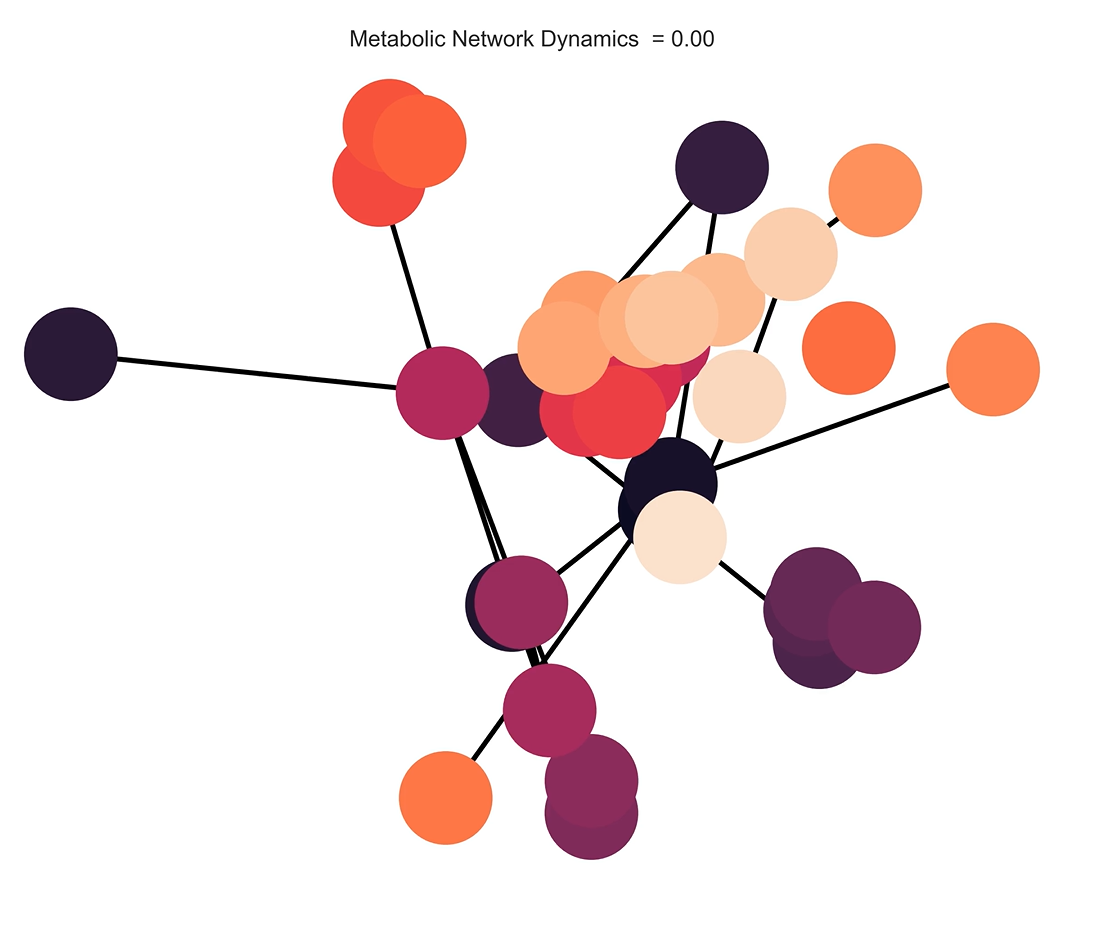
\includegraphics[width=0.5\linewidth]{s1.png}}
    
\end{figure}
\begin{figure}[H]
    \centering
   
    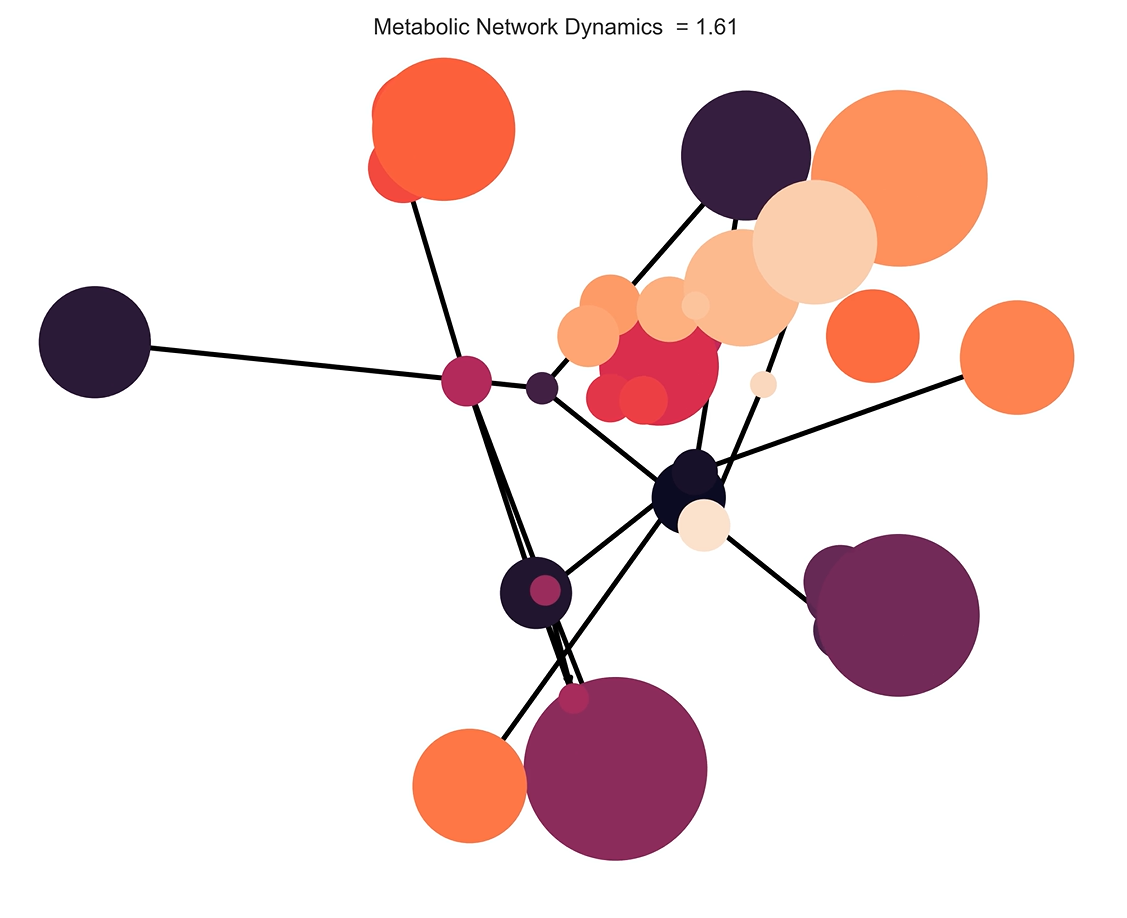
\includegraphics[width=0.5\linewidth]{s2.png}}
    
\end{figure}
\begin{figure}[H]
    \centering
   
    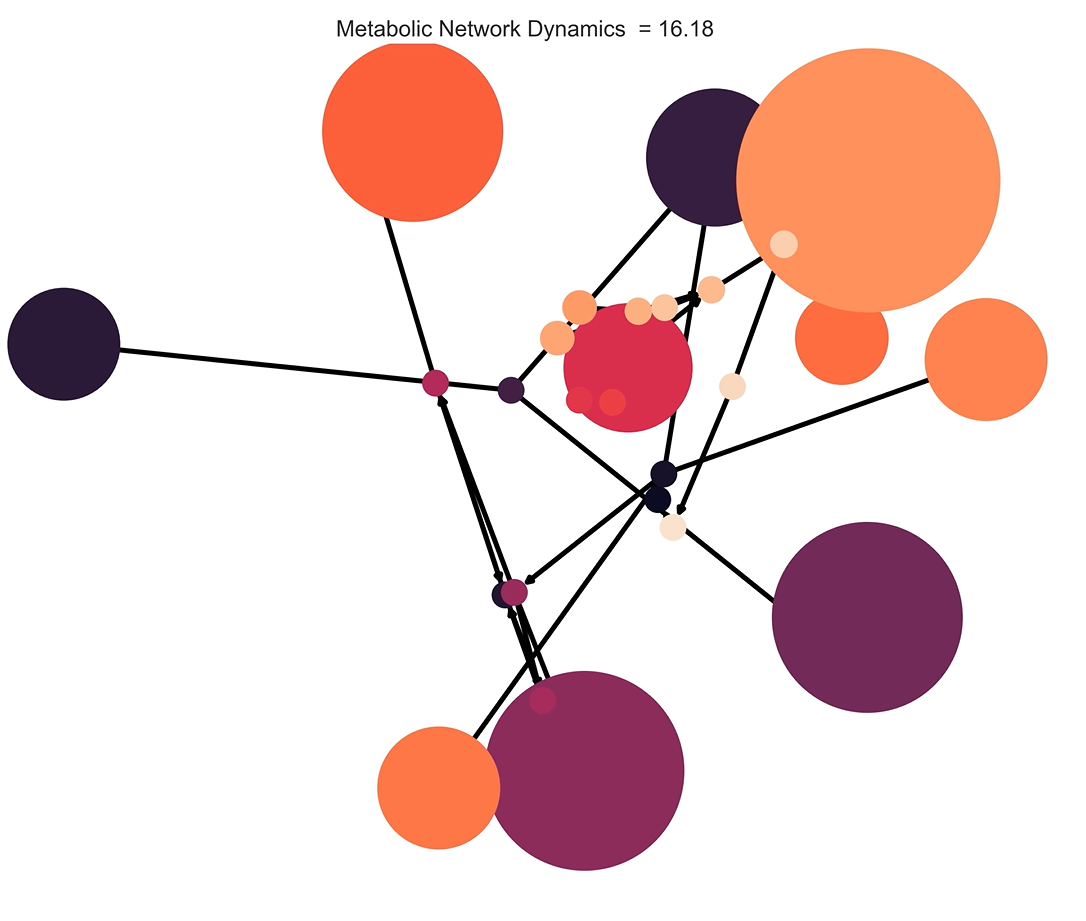
\includegraphics[width=0.5\linewidth]{s3.png}}
    
\end{figure}
\newpage
\textbf{Network2 Map00400}
\begin{figure}[H]
    \centering
   
    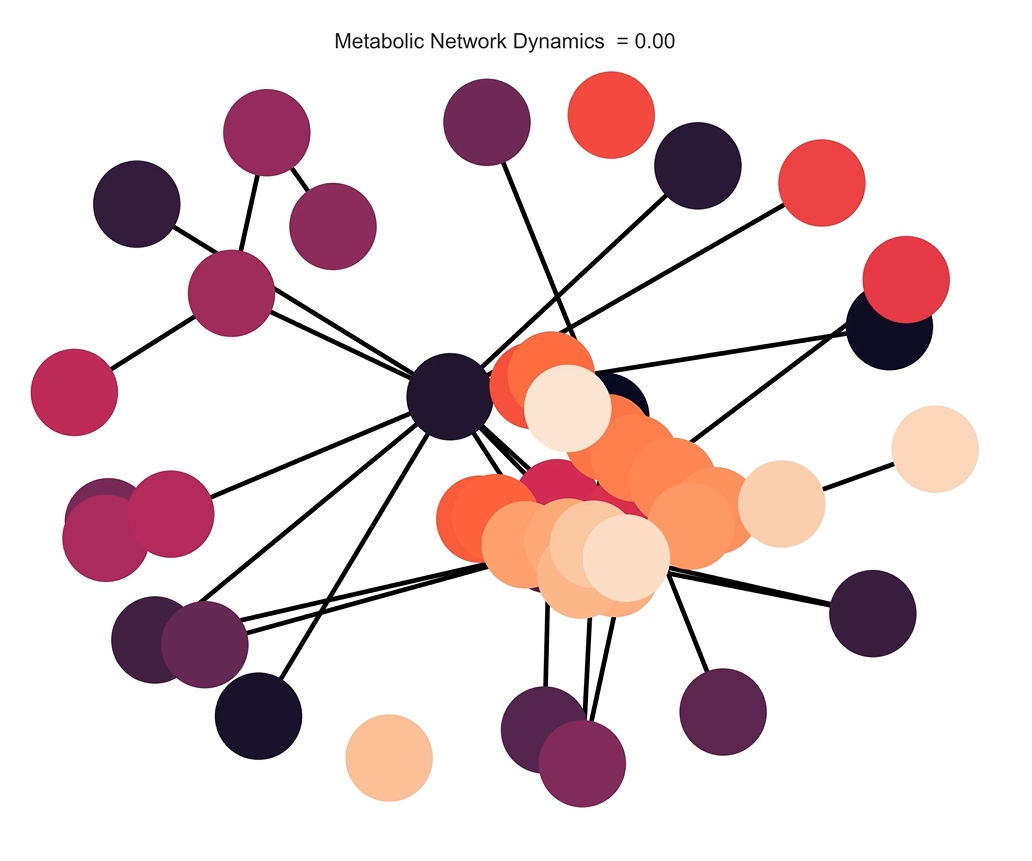
\includegraphics[width=0.5\linewidth]{V1.png}}
    
\end{figure}
\begin{figure}[H]
    \centering
   
    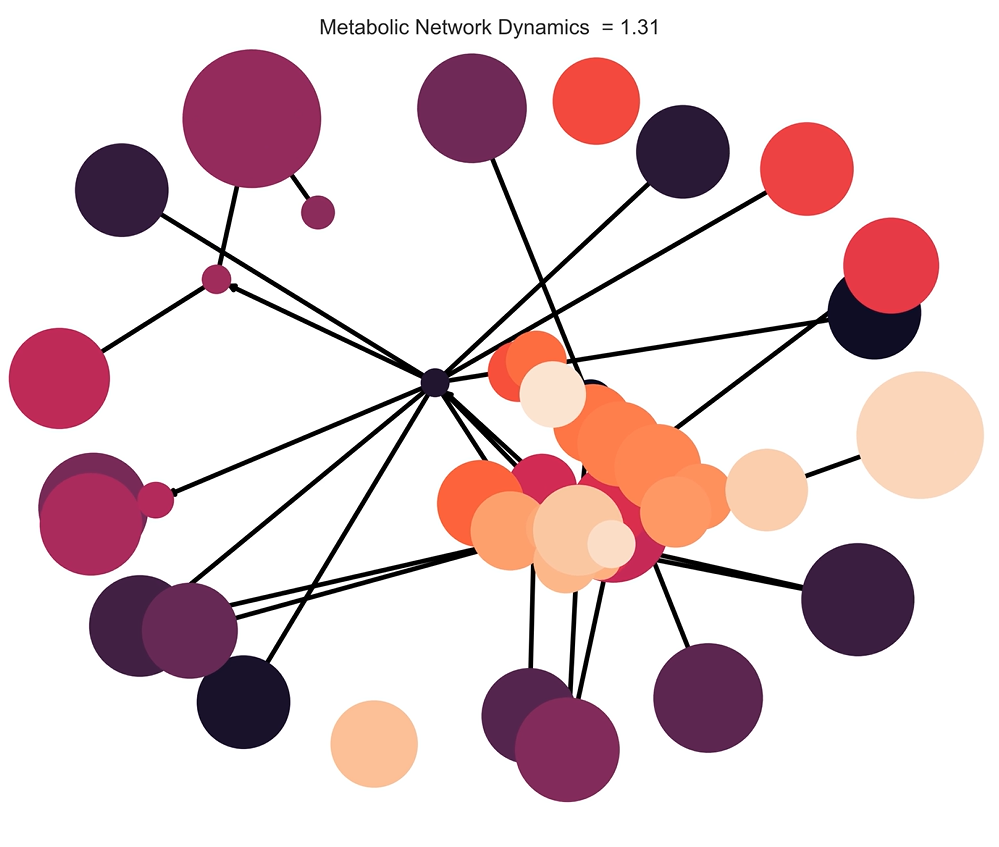
\includegraphics[width=0.5\linewidth]{V2.png}}
    
\end{figure}
\begin{figure}[H]
    \centering
   
    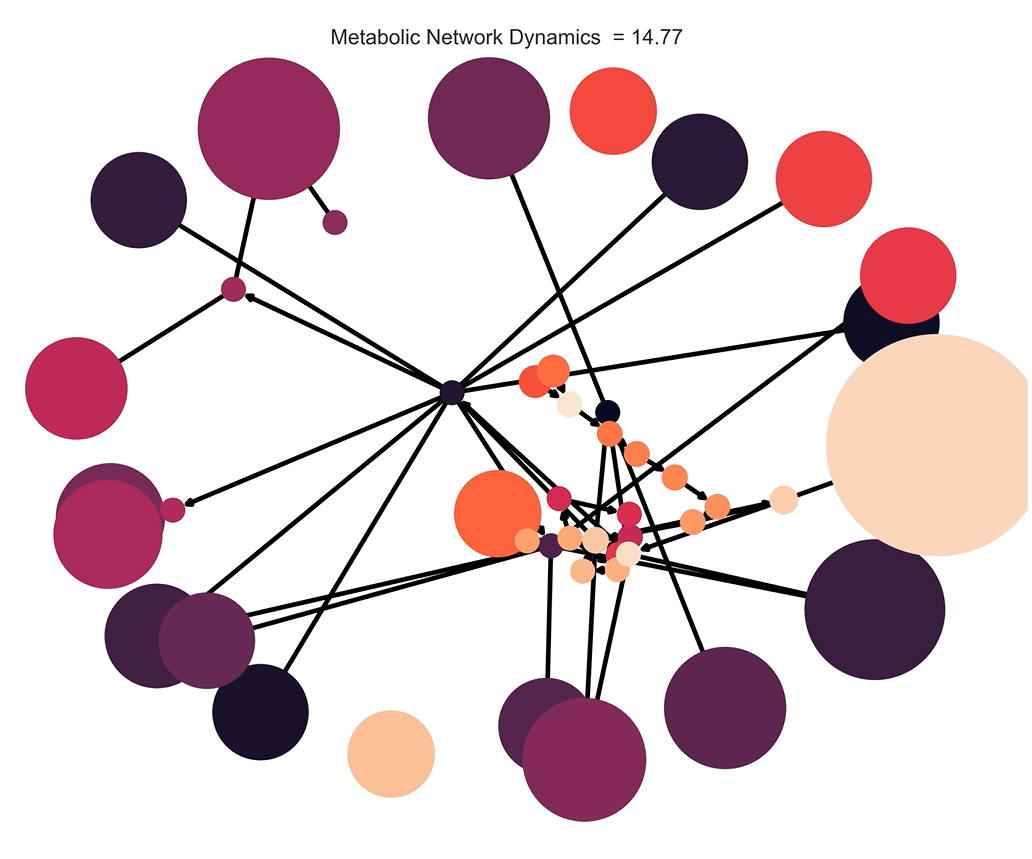
\includegraphics[width=0.5\linewidth]{V3.png}}
    
\end{figure}
\newpage
\section*{Theorising digital organisms}
I was thinking about how we can model digital organisms using networks, similar to biological systems, my planned digital organism, DIOR (digital organism) was a fun kind of project, mostly because i came across very complex research papers and i dropped the idea of making reality like digital organisms on my 12 GB RAM laptop. I say so because it took a whole year for a research team to move a single worm inside the screen. So my idea was to create DIOR using simple CRNs and keep text files as information and energy resources, we can have a virtual sun and a 2D grid for DIOR to live on. Let us dive deep on this Idea. \\
Here is a link to scientific paper titled \href{https://www.nature.com/articles/s41598-024-52475-9}{"Simulation of the emergence of cell-like morphologies with evolutionary potential based on virtual molecular interactions"} \\
\textbf{Abstract:} This study explored the emergence of life using a simulation model approach. The “multiset chemical lattice model” allows the placement of virtual molecules of multiple types in each lattice cell in a two-dimensional space. This model was capable of describing a wide variety of states and interactions, such as the diffusion, chemical reaction, and polymerization of virtual molecules, in a limited number of lattice cell spaces. Moreover, this model was capable of describing a wide variety of states and interactions, even in the limited lattice cell space of 100 × 100 cells. In this study, I assumed 18 types of virtual molecules, i.e., 18 virtual numbers that do not correspond to real molecules with chemical reactions represented by transformation of the numbers that occur with a specified reaction rate probability. Furthermore, it considered the energy metabolism and energy resources in the environment, and was able to reproduce “evolution,” in which a certain cell-like shape that adapted to the environment survived under conditions of decreasing amounts of energy resources in the environment. This enabled the simulation of the emergence of cell-like shapes with the four minimum cellular requirements, i.e., boundary, metabolism, replication, and evolution, based solely on the interaction of virtual molecules.
\\
Ishida (2024) used a 100 X 100 lattice of virtual molecules that diffuse, react and polymerise. His model showed that cell like shapes could spontaneously form with basic life features such as bounday, metabolism, replication and evolution. In his model, molecules of different types transformed stochastically simulating chemical reactions and it could contain a informational ploymer molecule through cell divisions. The model even included a form of energy metabolism, when energy resources in the environment were scarce, only certain shapes survived having a certain polymer and reproduced, which demonstrates an emergent evolutionary process. Attached snapshot from his paper, illustrates his multiset chemical model. \\
\begin{figure}[H]
    \centering
   
    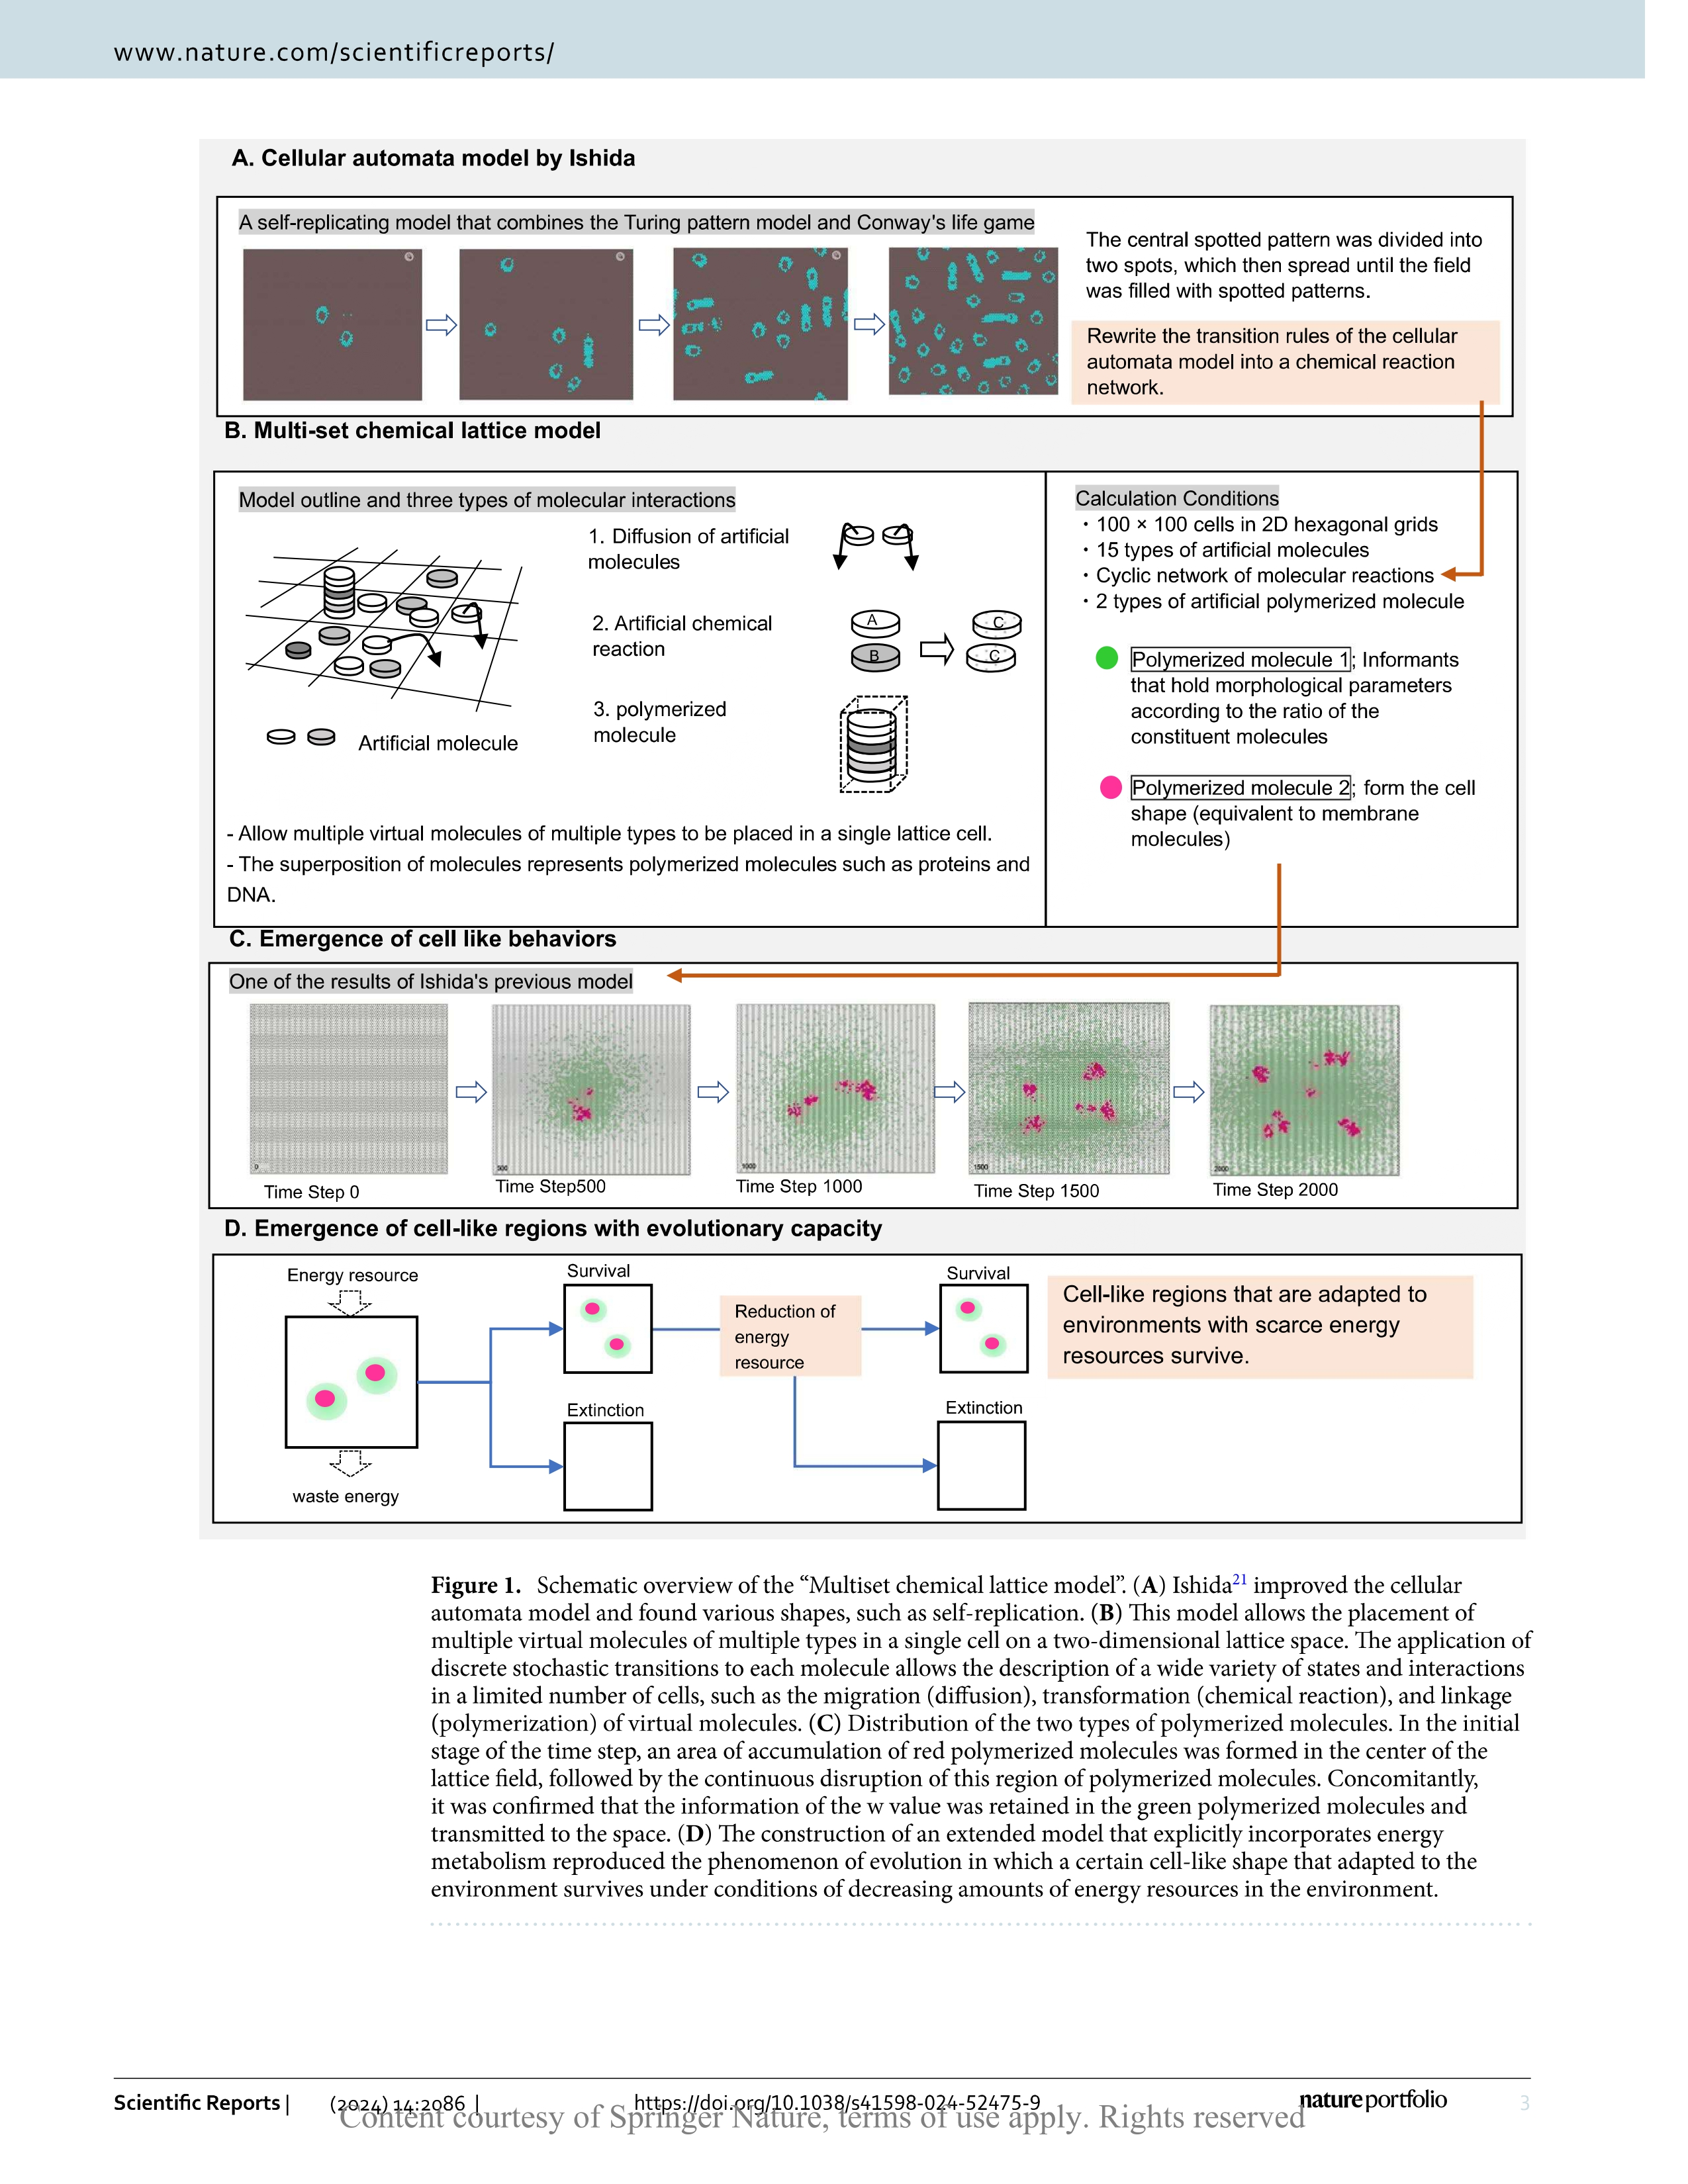
\includegraphics[width=1\linewidth]{save_page-0001.jpg}}
    
\end{figure}
\newpage
Development of such a system would take so much compute and time, the OpenWorm project (an attempt to simulate simple 1 mm worm) required many years of work and parallel team. In 2013 their team released only a rudimentray demo that showed just a few body parts moving and reported it would take another three to five months for a user friendly virtual worm was full runnable. Below is the 2019 docker container version for the worm. \\
\begin{figure}[H]
    \centering
   
    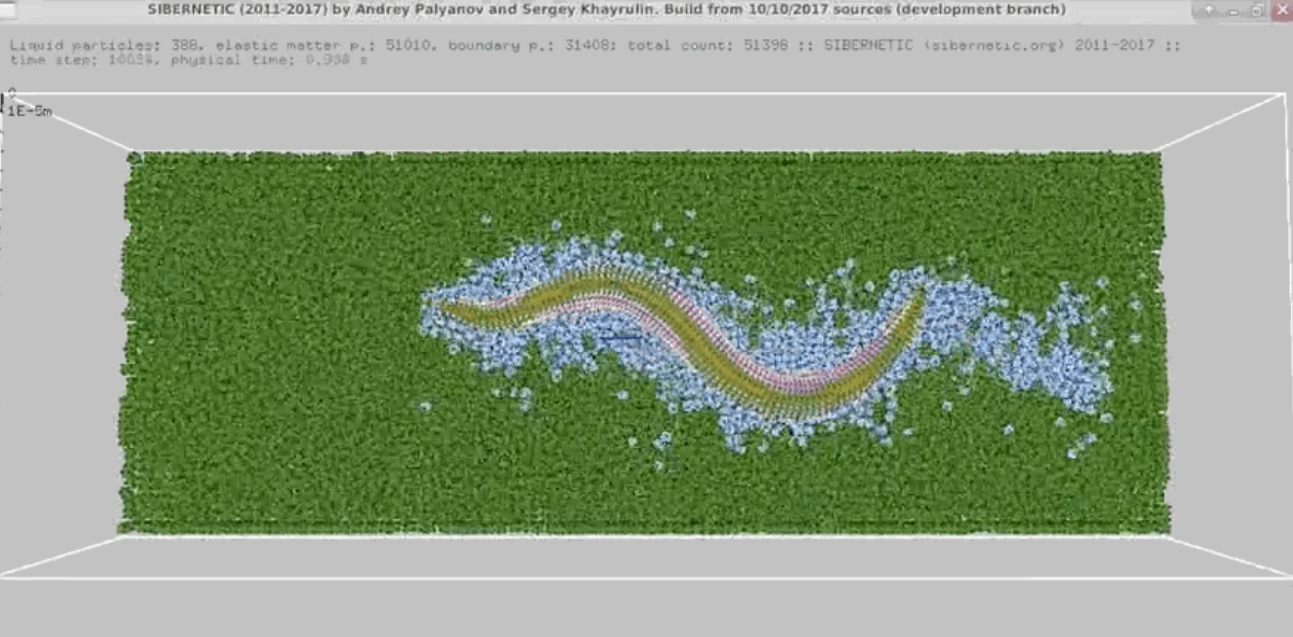
\includegraphics[width=1\linewidth]{worm.png}}
\end{figure}
So our system DIOR would be a very simplistic organism taking decisions based on certain chemical reaction networks, the system would need a 2D world grid with energy resources for example vritual sun that periodically adds energy and a way to let DIOR eat resources (.txt files in our case). Many digital life platforms treat CPU time as energy, for example in Avida system each organism gets CPU cycle to runs its individual code and performing tasks yield extra cycle to run, anaologous to metabolizing food. We can simply credit DIOR with energy points when it ingests a text file. Another feature can be penalizing damage, for example if it runs out of energy or collides then it dies or loses health points. We can include asexual reporduction once DIOR reaches certain enrgy points. Our model needs to simple and complex at the same time, for example DIOR eats .txt files then it itself gets stored as a .txt file (or JSON/.cvs as there are more code friendly) so that it can be eaten up by its descendants when no other .txt file is available. We need to have just the necessary variables, to simulate full isolation and behaviour of DIOR.\\
I am not too optimistic about this idea but we would try to do something experimental with the next biweekly report.
\section*{Discussion and Future Work}
In this report we have improved our dynamic comparison framework and took a step towards something fun and exciting, an inside the screen organism. This idea is fun because its make us seat on the god seat, the creator's seat. But we still have some pending work from previous weekly reports and future improvements on this report as well.
Our working code now can handle any two kgml files and output persistence diagram, graph maps, dynamic comparison metrics, overlay graphs and animated visualizations. However, there are still several avenues for further enhancement and validation:
\begin{itemize}
    \item Implementing proper parameter estimation methods to calculate rate constants from literature or related databases to increase biological realism of dynamic simulations.
    \item Expanding the dynamic comparison framework to include stochastic simulation algorithms (e.g., Gillespie) to capture intrinsic noise in biochemical networks.
    \item Writing more theory and Developing  DIOR (digital organism) prototype using simplified CRNs and energy/resource management within a 2D grid environment.
    \item Agenda items of biweekly report 2 (comparing permutations
    of the KGML files using API of KEGG databases or easier version of this
    could be , we can save 100s of KGML files in a specific folder, than our script compares
    these 100 files with each other that would be 4950 comparisons, and return to us just those
    files that fit our criteria of similarity.) and others listed in Biweely Report 2.
\end{itemize}
\begin{table}[H]
    \centering
    \begin{tabular}{ccc}
        Event & Timeline \\
        Biweekly Report 1 & 21 August  \\
        Biweekly Report 1.1 &  25 August \\
        Mid semester exams &  1-2 September \\
        Biweekly Report 2 & \sout{3 September} 7 September  \\
        Mid semester exams &  \sout{3 September}  10 September  \\
        Awaiting Feedback &   September-October \\
        Mid semester II exams &    10-16 October \\
        Biweekly Report 3 &  \sout{21 September} 24 October  \\
        Biweekly Report 4 & 7 November \\

    \end{tabular}
    \label{tab:placeholder}
\end{table}
\vfill
\noindent{\small Generated: \today}

\end{document}
